\chapter{Realisierung der clientseitigen Implementierung als Webapplikation}
\label{cha:web-app}
In diesem Kapitel wird die Implementierung des Clients als Web-Applikation. Hierbei wird auf die verschiedenen Design-Entscheidungen und genutzten Techniken näher eingegangen. 
\section{Definition einer Single Page Application}
\label{sec:Definition-SPA}
Die Web-Applikation wurde als \ac{Single Page-Application}(SPA) implementiert. \\Bei diese Art der Webanwendung wird die Verarbeitung von Anfragen vom Server auf die Client verschoben. Die daraus entstehende Anwendung benutzt nur wenige statische Hauptseiten, um den Inhalt darzustellen. Alle dynamischen Inhalte der Seite werden nachträglich per AJAX-Requests hinzugeladen.  Hierbei wird die Verarbeitung der nachgeladenen Daten auf dem Client durchgeführt und anschließend in die vorhandene HTML-Struktur übernommen, wobei der Grad der Autonomie des Clients vom genutzten Framework abhängt. Diese Auslagerung der Verarbeitung begünstigt die Nutzung des RESTful Webservices (siehe Kapitel \ref{cha:server-impl}), welcher die Daten liefert, die die SPA dann verarbeiten kann. Daraus ergibt sich, dass die Verbindung zum Server nur lose vorhanden ist. Es müssen nur  die wenigen statischen Seiten und deren eingebundenen Skripten vom Server abgerufen werden. Die sonstige Kommunikation besteht nur noch zwischen der SPA und dem Webservice. Im Laufe diese Kapitels wird noch darauf eingegangen, wie auch diese beiden Verbindungen durch geeignete Techniken bis auf ein Mindestmaß reduziert wurden.\footcite[S. 31f.]{book:AngularJs:Steyer2015}
\section{AngularJs}
\label{sec:AngularJs}
Zur Umsetzung der SPA wurde das quelloffene Framework AngularJs from Google gewählt, welches sich immer größerer Popularität erfreut\footcite{online:angularjs-popularity}\footcite[S. 33]{book:AngularJs:Steyer2015}. Es bietet alle Möglichkeiten, um einen Endgerät als weitestgehend autonomen \ac{Fat-Client} zu implementieren. Dadurch wird die Möglichkeit geschaffen, eine Applikation zu entwickelte, welche selbst dann akzeptabel reagiert, wenn ein aufrufendes Endgerät keine Verbindung zum Internet besitzt. Hierzu stellt es zusätzliches \ac{MarkUp} bereit, welches zu Laufzeit interpretiert und ausgeführt wird. Die dazu nötigen Komponenten von AngularJs und deren Einsatz werden nachfolgend genauer erläutert.

\subsection{Begriff: Komponente}
Wenn in diesem Kapitel der Begriff Komponente benutzt wird, ist eine abgeschlossene, logische Einheit im AngularJs-Umfeld gemeint. Auf einige dieser Komponenten, wie Services und Controller, wird im späteren Verlauf dieses Kapitels detaillierter eingegangen. AngularJs nutzt den Begriff des \textit{Modules} als einen Container für verschiedene Komponenten\footcite{online:angular:module}. 
\subsection{Dependency Injection}
\label{ssec:SPA-Dependency-Injection}
AngularJs wurde so konstruiert, dass zu jeden Zeitpunkt eine gute Testbarkeit gewährleistet ist. Aus diesem Grund setzt AngularJs für die Verbindung von verschiedenen Funktionen auf \textit{Dependency Injection}. \\ Hierbei wird beim Ausführen einer Funktion die genutzten Parametern geprüft. Gibt es eine bekannte Komponente, welche den gleichen Namen, wie der geforderte Parameter besitzt, erzeugt AngularJs ein Objekt diese Komponente und übergibt dieses an die Funktion. Hierbei wird bei der Erzeugung der Objekte für die Parameter ebenfalls Dependency Injection angewandt.\footcite{online:angularjs:dependency-injection}
\subsection{Services}
\label{ssec:SPA-Services}
Services sind abgeschlossene Komponenten, welche bestimmte Funktionalitäten kapselt und bereitstellen. AngularJs bietet neben der Möglichkeit, eigene Services zu erstellen eine große Auswahl an vorhandenen Services, um verschiedene wiederkehrende Aufgaben durchzuführen. Dabei sind die Services von AngularJs immer mit dem Präfix \textit{\$} versehen. Einer der wichtigsten Serviceses für die Umsetzung dieser Arbeit war beispielsweise \$http. Dieser stellt Funktionen bereit, welche zur Kommunikation eines Web Services mittels HTTP benötigt werden. \\
Services können von Controllern (siehe \ref{ssec:SPA-MVC}) verwendet werden, um Daten zu erhalten und an die Oberfläche weiterzugeben. Hierbei verwenden Sie \textit{Dependency Injection}, um auf einen Service zuzugreifen, wobei nur beim ersten Zugriff ein neues Objekt erzeugt wird (\ac{Singleton}-Muster). Fordert eine weitere Komponente ein Objekt des Services, wird das bereits erstellt Objekt zurückgegeben. \footcite{online:angular:services}
\subsection{Promises}
\label{ssec:SPA-Promises}
Im letzten Abschnitt wurde der Service \textit{\$http} angesprochen (siehe \ref{ssec:SPA-Services}), welches Methoden zur Kommunikation mit einem RESTful Webservice bereitstellt. Würde diese Kommunikation synchron ausgeführt werden, würde diese AngularJs bis zum Erhalt der Antwort blockieren, da Javascript immer nur in einem Thread ausgeführt wird\footcite{online:javascript:single-threaded}. Deshalb wurde das Prinzip der \textit{Promises} eingeführt. Dies erlaubt die Abarbeitung von asynchronem Code, indem beim Aufrufen einer asynchron abzuarbeitenden Methode ein \textit{Promise}-Objekt zurückgegeben wird. Die repräsentiert ein Versprechen über einen späteres Ergebnis. Auf dieses Ergebnis kann mit den Methoden \textit{then} und \textit{catch} reagiert werden. \textit{Then} wird nach erfolgreicher Abarbeitung der asynchronen Methode ausgeführt. Tritt bei der Verarbeitung ein Fehler auf, wird die \textit{catch}-Methode ausgeführt. Da diese beiden Methoden jeweils selber Promise-Objekte zurückgeben, ist ein verketten der Aufrufe möglich. 
Die Nutzung von Promisses ist im \textit{Module} \textit{\$q} gekapselt, welches sich an dem Projekt \textit{q} orientiert. 
\footcite{online:angular:module:q} 
\footcite{online:doc_q} 
\footcite[S. 211ff]{book:AngularJs:Steyer2015}.
\subsection{MVC}
\label{ssec:SPA-MVC}
AngularJS nutzt das Architektur-Muster \ac{MVC} um Datenbeschaffung bzw. -haltung, Datenverarbeitung und Datenpräsentation strikt zu trennen. \\ 
Zur Beschaffung werden entweder Services, welche per Dependency Injection hinzugeladen werden, benutzt oder Model-Funktionen erstellt, welche mit Konstruktoren aus dem objektorientierten Umfeld verglichen werden können. \\
Die so erhaltenen Datenstrukturen können von Controllern aufgerufen werden. Dabei handelt es sich um Komponenten, welche von AngularJs zur Anreicherung eines bestimmten MarkUp-Blocks aufgerufen werden. Ihre Aufgabe ist es, die für die Oberfläche benötigten Daten zu besorgen, diese aufzubereiten und sie an die View weiterzugeben. Das Code-Beispiel \ref{lst:SPA-controller-navigation} zeigt den Aufbau einer Controller-Komponente, welche Daten für die Navigationsleiste bereit stellt\footcite{online:angular:controller}.
\lstinputlisting[caption=Controller für die Navigationsleiste, label=lst:SPA-controller-navigation, style=htmlcssjs]{content/listings/indexcontroller.js}
Hierbei ist zu sehen, wie mittels \textit{Dependency Injection} die benötigten Komponenten für die Funktion bereitgestellt werden (Zeile \ref{line:controller:dependency-injection}). Interessant ist dabei besonders die Komponente \textit{\$scope}. Diese wird verwendet, um Daten zwischen dem Controller und der View (in dem Fall der statischen HTML-Seite) auszutauschen (Zeile \ref{line:controller:scope}ff.)\footcite{online:angular:scopes}. Dabei stellt AngularJs Funktionen bereit, um diesen Austausch bidirektional durchzuführen. Somit können beispielsweise Daten, welche ein Nutzer in ein Textfeld eingibt, im Controller weiter verarbeitet werden.\\
Die Benutzung der durch den \textit{\$scope} bereitgestellten Variablen wird im Beispiel \ref{lst:SPA-navigation} gezeigt.\\
\lstinputlisting[caption=Navigation der Hauptseite erweitert um AngularJS-MarkUp, label=lst:SPA-navigation, style=htmlcssjs]{content/listings/Index.html}
Über das Attribute \textit{data-ng-controller} (Zeile \ref{line:indexHtml:controller}) wird ausgesagt, dass dieser \textit{div}-Block durch die Controller-Funktion \textit{indexController} bearbeitet wird. Nur in diesem Geltungsbereich kann auf die Eigenschaften des Controllers zugegriffen werden. \\
Hierbei gibt es verschiedene Möglichkeiten, die Daten des Controllers zu benutzten: 
\begin{itemize}
\item \textbf{Nutzung in Direktiven}\\
AngularJs stellt Direktiven bereit, welche die Darstellung der Webseite beeinflussen. Dies zeigt sich in Zeile \ref{line:indexHtml:Nutzung_Direktive}. Das Direktiv \textit{ng-hide} wird benutzt, um dynamisch HTML-Element auszublenden. Um zu entscheiden, ob das zugehörige \textit{li}-Element ausgeblendet werden soll, wird die Variable \textit{onlineStatus} aus dem \textit{\$Scope} des Controllers abgefragt. Ändert sich die Variable im Controller, wird die Direktive neu ausgewertet\footcite{online:angular:diretive}.
\item \textbf{Ausgabe des Wertes}\\
Der Wert einer Variable kann direkt ausgegeben werden. Dies wird in Zeile \ref{line:indexHtml:Nutzung_Variable} gezeigt. Damit AngularJs erkennt, dass eine \textit{\$scope}-Variable ausgegeben werden soll, muss diese von zwei geschweifte Klammern umgeben sein.
\item \textbf{Zugriff auf Methoden}\\
In Zeile \ref{line:indexHtml:Nutzung_Methode} wird eine Direktive benutzt, um aus der View heraus eine im \textit{\$scope} definierte Funktion aufzurufen.
\end{itemize}
\subsection{Routing}
\label{ssec:SPA-Routing}
Damit das MarkUp nicht schnell durch die Nutzung von zusätzliche Direktiven überladen wird, bietet AngularJs das module \textit{\$route} zur Implementierug von Routing an. Hierbei wird durch die Direktive \textit{ng-view} ein Block als View-Container definiert. Dieser wird abhängig von der aufgerufenen URL mit unterschiedlichen Inhalten befüllt. Das Beispiel \ref{lst:SPA-routing} zeigt solch eine Routing-Konfiguration. 
\lstinputlisting[caption=Routing mit AngularJs, label=lst:SPA-routing, style=htmlcssjs]{content/listings/routing.js}
Stimmt eine Route überein wird der konfigurierte Controller aufgerufen. Dessen Scope wird nach der Abarbeitung an die definierte View weitergegeben. Die Views sind hierbei Html-Dateien mit MarkUp-Schnipsel, innerhalb des View-Containers gerendert werden. Diese MarkUp-Schnipsel liegen ebenfalls auf dem Server. 
\section{Umsetzung}
\label{sec:SPA-Umsetzung}
Durch die Nutzung der vorgestellten Komponenten war es möglich, einen Prototyp, welcher die grundlegenden Anforderungen, die in Kapitel ((ANFORDERUNGEN)) definiert wurden, erfüllt.\footcite{online:Created_SPA} Nachfolgend werden einige Teilaspekte im Zusammenhang mit der Implementierung näher beleuchtet.
\subsection{Layout mit Twitter Bootstrap}
\label{ssec:SPA-twitter-bootstrap}
Zur Erstellung einer Oberfläche wurde vollständig auf das bewehrte, quelloffene CSS-Framework \textit{Bootstrap} von Twitter gesetzt. Dies ist unter dem Aspekt designet, einmal definiertes CSS auf allen Endgeräten eine natürliche und gut nutzbare Anwendung entsteht. Dies liegt daran, dass \textit{Bootstrap} es erlaubt, unter Nutzung eines integrierten Grid-Systems eine hoch-responsive Applikation zu erstellen.\footcite{online:get-bootstrap}\\
Durch den großen Umfang des Frameworks und da im ersten Schritt nur ein Prototyp erzeugt werden sollte, war es möglich, alle Anforderungen in die Web-Applikation zu integrieren ohne, dass weitere Implementierung von CSS nötig war.

\subsection{Herausforderung statusloses Protokol Http}
\label{ssec:statusloses-http}
Da HTTP ein statusloses Protokol ist, ist es ohne Weiteres nicht möglich, ein einmal abgerufenes Access-Token wiederzuverwenden. Um dies dennoch zu erreichen, wurde Service \textit{authFactory} entwickelt, welcher sich um das ein- und ausloggen kümmert. Hierbei wird unter Zuhilfenahme der \textit{LocalStorage}-Api ein erhaltenes Access-Token mit dem Nutzernamen und dem Ablaufdatum persistiert. Ist dieser Datensatz vorhanden und das Ablaufdatum noch nicht erreicht, gilt der Nutzer als angemeldet und kann auf seine Trainingspläne zugreifen. \\
Gleichzeitig wird für die Verwaltung von Inhalt, welchen nur authentifizierte Nutzer abrufen können eine weitere Komponente benutzt, nämlich der \textit{Interceptor}. Dies ist ein spezieller Service, welcher eng mit dem \textit{\$http}-Service verbunden ist. Mit dem Interceptor ist es möglich, eine Request kurz vor- und eine Response direkt nach Erhalt einzusehen und gegebenenfalls darauf zu reagieren. Dies wird verwendet, um vor dem Absenden eines Request den \textit{authorizsation}-Header zu setzen, falls ein Access-Token vorhanden ist. \\ Der Respond ist wegen des eingehenden Statuscodes interessant: Wenn der Web Service mit \textit{401 (Unauthorised)} antwortet, ist der Nutzer nicht angemeldet. Daraufhin wird ein möglicher Datensatz mit einem Access-Token gelöscht und der Nutzer wird auf die Login-Seite umgeleitet\footcite{online:Created_SPA}. 

\subsection{Online-Check}
\label{ssec:Online-Check}
Der Nutzer soll eine visuelle Rückmeldung darüber bekommen, ob die Applikation gerade eine Verbindung zu Web Service aufbauen kann oder nicht. Dafür wurde der im Beispiel \ref{lst:SPA-controller-navigation} gezeigte Controller um einen Online-Check erweitert. Ruft die Anwendungen in einem 5 Sekunden-Intervall die URI \textit{http://fit-bachelor.azurewebsites.net/api/accounts/ping}. Schlägt diese Anfrage mit den Statuscode \textit{0} fehlt, liegt keine Verbindung vor und der aktuelle Status ändert sich von \textit{Online} zu \textit{Offline}.
\begin{figure}[h]
\centering

\includegraphics[width=0.8\linewidth]{content/images/SPA-Online-Check}
\caption{Screenshot: Veränderung der Statusanzeige, wenn keine Verbindung zum Internet besteht}
\label{pic:SPA:OnlineCheck:Statusänderung}
\end{figure}

\section{Erweiterung um Offline-Nutzung}
\label{sec:CachedHttpService}
Die bisher vorstellten Komponenten um Umsetzungen führten zum Prototyp einer funktionierenden Single Page Applikation. Diese benötigt aber zur Nutzung noch eine Verbindung zum Webserver, auf der die Applikation gehostet wird und eine Verbindung zum Web Service, zur Durchführung von Interaktionen. In den folgenden Abschnitten wird beschrieben, wie Techniken eingesetzt wurde, um den Zugriff auf diese Ressourcen auf ein Minimum zu reduzieren. 
\subsection{Implementierung des CachedHttpServices}
\label{ssec:Implementierung-cachedHttpService}
Zur Reduzierung der Bindung an den Webservice wurde ein Cache implementiert. Hierbei wurde von der Planung des Caches aus Kapitel ((CACHE BESCHREIBUNG)) abgewichen. \\
Eigentlich sollte für jede Entität ein lokales Pendant erstellt werden, welche die Daten speichert, die bei einem Verbindungsabbruch nicht an den Server gesendet werden können. Durch die besonderen Eigenschaften von JavaScript und der genutzten Datenbank war eine Vereinfachung dieser Planung möglich:
\begin{itemize}
\item Javascript erlaubt es, Objekt zur Laufzeit beliebig zu verändern und zu erweitern. Darum kam die Idee auf, die Serverdaten, welche noch nicht an den Server gesendet wurde um Meta-Daten für die lokale Speicherung zu erweitern und anschließend lokal zu persistieren.
\item Diese Möglichkeit wird durch die Datenbank unterstützt. Es handelt sich dabei um die \textit{Indexed Database API}. Diese erlaubt es, innerhalb des Browsers eine \ac{NoSQL}-Datenbank anzulegen und zu verwalten. Sie wird von den meisten Browsern unterstützt\footcite{online:caniuse:indexedDB}. Da \textit{NoSQL}-Datenbanken keine festen Schema kennen, sondern beliebige Datenstrukturen per Index oder Schlüssel bestimmt, ist die Ablage eines dynamisch erstellten Objekts ohne weiteren Aufwand möglich. Zur Nutzung der IndexedDB wurde ein externes AngularJs-Module verwendet.\footcite{online:AngularJs:indexedDB}
\end{itemize}  
Durch diese Änderungen kann die Erstellung des lokalen Caches erheblich vereinfacht werden, indem nicht mehr für jede Entität ein lokales Abbild vorgehalten wird. Es gibt eine zentrale Stelle für DB-Entitäten, welche wie folgt aussieht.

\begin{figure}[h]
\centering
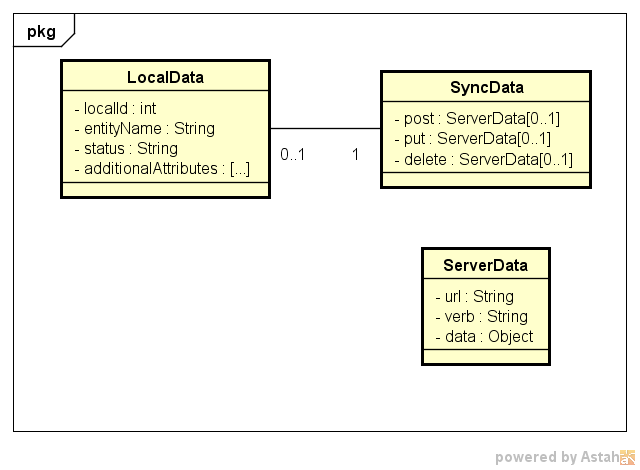
\includegraphics[width=0.8\linewidth]{content/images/DataModel-Cache-SPA}
\caption{Screenshot: Datenmodel zur Speicherung lokaler Daten}
\label{pic:DataModel-Cache-SPA}
\end{figure}

\subsubsection*{Umsetzung des Caches über HTTP-Verbs}
\label{sssec:Http-Verbs}
Durch diese Zentralisierung der Cache-Daten konnte ein Service entwickelt werden, der den \textit{\$http}-Service kapselt und bei jedem Senden einer \textit{GET}-, \textit{POST}-, \textit{PUT}- und \textit{DELETE}-Anfrage die lokalen Daten mit denen des Web Services synchronisiert. Dafür wird nach dem Senden der Nachricht geprüft, ob der Web Service erfolgreich erreicht wurde.\\
Ist dies der Fall, werden die neuen Daten mit dem Status \textit{Server} lokal aktualisiert. Dies sagt aus, dass die Daten mit denen des Servers übereinstimmen und keine Synchronisation erfolgen muss.\\
Wenn der Web Service nicht erreicht wurde, werden die Daten mit dem Status \textit{local} zwischen gespeichert. Dazu wird ein \textit{SyncData}-Objekt unterhalb des lokalen Datensatzes angelegt. Dieses definiert Eigenschaften mit Daten für spätere Synchronisationsprozesse.

\subsubsection*{Synchronisation zwischen Server und SPA}
\label{ssec:Sync-SPA}
Ist der Web Service wieder erreichbar, werden alle Datensätze mit dem Status \textit{local} synchronisiert, indem die Anfragen nacheinander an den Server gesendet werden. \\Hierbei wird per Verb entschieden, welche Methode des \textit{\$http}-Services genutzt werden soll. Dieser werden dann die gespeicherte URL sowie eventuelle Daten zum Senden an den Server übergeben. \\
Die Reihenfolge der verarbeiteten HTTP-Verben für die Synchronisation wurde wie folgt gewählt:
\begin{itemize}
\item \textit{DELETE}\\
Besitzt ein Objekt einen offene Delete-Befehl, wird dieser als erstes durchgeführt. Alle weiteren offenen Synchronisationsprozesse werden im Zuge der Löschung dieses Datensatzes ebenfalls mit gelöscht. Dadurch wird die Anzahl der benötigten Requests verringert. \\Kommt es bei einem Objekt zu einem Create/Post- und Delete-Request, ohne, dass zwischenzeitlich eine Synchronisation durchgeführt wurde, wird der Datensatz direkt lokal gelöscht, ohne, dass Anfragen an den Server gesendet werden müssen. Dies dient ebenfalls der Verringerung der zu sendenden Requests. 
\item \textit{POST} \\
Sind keine \textit{Delete}-Requests vorhanden, wird nach einem offenen POST-Request für das Objekt gesucht. Dieser wird dann durchgeführt. Mit dem Ergebnis wird die ID des lokalen Datensatzes angepasst, damit eventuell anstehende Update/Put-Requests auf das richtige Server-Objekt angewandt werden.
\item \textit{PUT} \\
Zum Schluss wird auf offene Put-Requests geprüft und gegebenenfalls durchgeführt. 
\end{itemize}
Nach jeder erfolgreichen Abarbeitung eines Synchronisationsprozesses, wird dieser aus dem Synchronisationsobjekt entfernt. Wenn dieses daraufhin keine offenen Prozesse mehr besitzt, wird es gelöscht. 
Damit der Nutzer nicht auf die Abarbeitung der Synchronisationsprozesse warten muss, wird dieser Vorgang komplett asynchron durchgeführt. Durch diese Änderungen ist eine Verbindung zum Webservice optional.

\subsection{Das AppCache-Manifest}
\label{ssec:appcache-manifest}
Der Einsatz des \textit{cachedHttpService} erlaubt eine Nutzung der \textit{SPA} auch ohne, dass eine Verbindung zum Web Service besteht. Doch noch braucht die \textit{SPA} eine Verbindung zu ihrem Host, damit statische Dateien wie \textit{View}-Templates und \textit{Script}-Dateien nachgeladen werden können. Diese Verbindungen können durch die Nutzung eines AppCaches stark reduziert werden. \\
Der \textit{AppCache} wurde im Zuge von \textit{HTML5} implementiert und wird von allen gängigen Browsern in der aktuellen Version unterstützt\footcite{online:caniuse:appcache}. Hierbei wird eine Manifest-Datei auf dem Server abgelegt, welche Aussagen darüber trifft, welche Dateien lokal auf einem Client gespeichert werden sollen. Im Falle dieser Arbeit wurde konfiguriert, dass alle Dateien lokal gespeichert werden (siehe Beispiel \ref{lst:SPA-appcache-manifest} ab Zeile \ref{line:appcache:local}ff.). 

\lstinputlisting[caption=Cache-Manifest-Datei, label=lst:SPA-appcache-manifest, style=htmlcssjs]{content/listings/CacheManifest.appcache}

Sind diese Dateien erstmal auf dem Client gespeichert, werde sie genutzt, wenn keine Verbindung zu Server besteht. \\
Damit die Dateien trotzdem auf dem aktuellen Stand sind, wurde im \textit{SETTINGS}-Bereich definiert, dass die Online-Ressourcen vorrangig genutzt werden sollen (siehe Zeile \ref{line:appcache:prefer-online}). Dies wird aber trotzdem nicht von allen Browser berücksichtigt, darum gibt es einen Weg, den Client dazu zu zwingen, die Ressourcen erneut von Server abzurufen. Hierzu muss die Manifest-Datei angepasst werden. Wenn der Client das nächste Mal eine Verbindung zu Server aufbaut, wird die neue Manifest-Datei heruntergeladen. Dies für dazu, dass der Client alle lokalen Dateien invalidiert und sich die Dateien, welche das neue Manifest-Datei definiert, erneut herunterläd. Damit das aktualisieren der Datei leichter umgesetzt werden kann, wurde ein Zeitstempel als Kommentar in die Manifest-Datei integriert (siehe Zeile \ref{line:appcache:timestamp}). Somit kann man leicht ein Neuladen der Serverdateien herbeiführen. 
\section{Fazit}
Es konnte ein voll funktionsfähiger Prototyp entwickelt werden, welcher die Anforderungen aus für den Prototyp umgesetzt hat. Hierbei wurde der Funktionsumfang mit dem Chrome der Version 44.0.2403.157 getestet.

